\chapter{Theory}
\label{cha:theory}

% The main purpose of this chapter is to make it obvious for
% the reader that the report authors have made an effort to read
% up on related research and other information of relevance for
% the research questions. It is a question of trust. Can I as a
% reader rely on what the authors are saying? If it is obvious
% that the authors know the topic area well and clearly present
% their lessons learned, it raises the perceived quality of the
% entire report.

% After having read the theory chapter it shall be obvious for
% the reader that the research questions are both well
% formulated and relevant.

% The chapter must contain theory of use for the intended
% study, both in terms of technique and method. If a final thesis
% project is about the development of a new search engine for
% a certain application domain, the theory must bring up related
% work on search algorithms and related techniques, but also
% methods for evaluating search engines, including
% performance measures such as precision, accuracy and
% recall.

% The chapter shall be structured thematically, not per author.
% A good approach to making a review of scientific literature
% is to use \emph{Google Scholar} (which also has the useful function
% \emph{Cite}). By iterating between searching for articles and reading
% abstracts to find new terms to guide further searches, it is
% fairly straight forward to locate good and relevant
% information, such as \cite{test}.

% Having found a relevant article one can use the function for
% viewing other articles that have cited this particular article,
% and also go through the article’s own reference list. Among
% these articles on can often find other interesting articles and
% thus proceed further.

% It can also be a good idea to consider which sources seem
% most relevant for the problem area at hand. Are there any
% special conference or journal that often occurs one can search
% in more detail in lists of published articles from these venues
% in particular. One can also search for the web sites of
% important authors and investigate what they have published
% in general.

% This chapter is called either \emph{Theory, Related Work}, or
% \emph{Related Research}. Check with your supervisor.

\section{Web browsers and CEF}

Later in this paper, the implementation of a web browser within Openspace will be presented. But first, what a web browser is, the purpose of a web browser, a web browser's structure and some challenges that web browsers handles needs to be described.

For the sake of clarity, a web browser as discussed in this paper is a software application, or a part of one, that receives an arbitrary web resource in the form of an Uniform Resource Identifier (URI). \cite{jacobs2009uri} It then downloads this resource and presents it in an appropriate fashion.

\subsection{Structure}

I order to meet the requirements of a web browser and handling all the content that is should be supported according to the HTML 5 standard \cite{html}, a web browser becomes an application with a complicated structure. Among several things, media download, web rendering and user interaction should all happen in the same application. All this preferably with little to no delay and without disrupting any of the other tasks.

In the CEF and Chromium projects, the sollution is handling most tasks through a mutli-processes, multi threaded approach. \cite{cefusage} This allows multiple tasks to be handled simultaneously. A user's interactions should ideally not disrupt the playback of a video or a sound, for instance.

\todo[inline]{events?}
\todo[inline]{rendering?}
\todo[inline]{off screen rendering?}

\subsection{Executables in CEF}

\begin{figure}[h]\label{fig:processes}
\centering
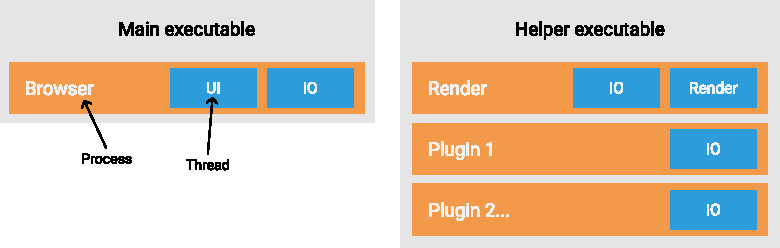
\includegraphics[width=0.9\linewidth]{./figures/process.pdf}
\caption{\emph{An overview of the two-executable structure with processes and threads.}}
\end{figure}

CEF has support for two different executable models. The implementation uses either one or two separate executables for its sub processes. An overview can be seen in figure \ref{fig:processes}. The processes are launched with different command line arguments that determine the purpose of the launched process. These arguments get sent to either the \texttt{CefExecuteProcess}, which then takes care of determining what needs to be done. The single-executable structure is supported on Windows and Linux system, but not on Macos systems. \cite{cefusage}

In a single-executable implementation of CEF, the return code of \texttt{CefExecuteProcess} is used to determine wether or not execution of that process should be terminated. In a two-executable implementation, the main executable (that also runs the rest of the application) initializes CEF with an option parameter declaring the location of the sub-process executable. In this case, the sub-executable is a single-purpose executable that does little else than calling \texttt{CefExecuteProcess} to allow CEF to handle the incoming task. By using dynamic, shared libraries, the double-executable approach does not necessarily increase the application size, as the two executables share the CEF library.

A potential drawback of a single-executable implementation is that the implementation becomes sensitive to where \texttt{CefExecuteProcess} gets called. If it is late in the application bootup, this may cause delays in CEF's sub-process spawning.

\subsection{Processes in CEF}

In CEF, each different thread and process have separate purposes. They handle different tasks. Although the there might be similarities between the tasks, they are distinct. The main, "browser", process handles window management (towards the host operating system), painting and network access. This process is the same as the host application, where the rest of the application's logic is run.

Another process is called the render process. This is where Blink rendering and javascript execution happens. Blink is Chromium's web rendering engine - it takes formatting information such as CSS style sheets and transform it into the visual result that eventually will be shown. \cite{blink} For safety and robustness, each unique combination of URL scheme and origin will trigger a new render process to be spawned. A URL scheme is the initial part of the URL, usually describing which protocol that should be used. It may look like \texttt{https}, \texttt{http} or \texttt{ftp}. The origin is in this case the domain name or IP address of the URL. By default, Chromium does not separate web pages from different sub domains (\texttt{one.example.com} and \texttt{two.example.com}) or ports (\texttt{example.com:80} and \texttt{example.com:443}). \cite{processes} This separation and reusability of processes is considered to give a good balance of safety and computing resource usage at the same time as allowing instances of different web pages from the same web site to access each other according to the enforced security policy. \cite{network10same}

The other processes that may be spawned by CEF are related to so called plugins. These might be if a web site wants to show content that are developed by a third party, for instance. This might be Flash content, Java aplets, or similar. GPU powered content are also being handled by a separate process.

An overview of the different processes together with its executables and threads can be seen in figure \ref{fig:processes}.

\subsection{Threads in CEF}

Each process in CEF is also multi threaded. This is where the multi-dimensional parallelism structure of CEF comes in. The different threads handle different aspects of constructing the requested web page. As mentioned in \cite{cefusage}, there are many different threads used by different processes. The most common ones are:

\begin{itemize}
  \item The \textbf{UI} thread. This is the main thread of the browser process. It is the thread where the function \texttt{CefInitialize} is called to initialize the CEF framework.
  \item The \textbf{IO} thread, where inter-process messaging is handled and where network messages are processed.
  \item The \textbf{renderer} thread, which is the main thread of the renderer process.
\end{itemize}

\subsection{Challenges}

\todo[inline]{write about challenges?}

\section{Web sockets}

The Web socket technology is an extension of TCP sockets made for two-way communication between a client and a host. The protocol uses TCP \cite{postel1981transmission} as the transport layer. By using HTTP to complete a handshaking process, a persistent connection between the peers may be established. This means that no further handshaking is required, since the TCP connection remains open. Web sockets are essentially a layer on top of TCP that adds web targeted security model, an addressing and naming mechanism to support several services on one port, a framing mechanism to describe the messages and some other more handshaking related mechanisms. \cite{fette2011websocket}

Arbitrary UTF-8 \cite{RFC3629} text messages or binary data may be sent over the connection. These are interpreted as standalone messages, and the peers should treat them as such. This differs from raw sockets where the messaging back and forth can be seen as streams, and where some sort of breaking character or sequence must be used to distinguish messages from each other. The web socket frame header contains details of how long the message is, and this tells the clients how to interpret the received frames and where the frames end.

Web socket supports both unencrypted messages with the URI scheme \texttt{ws://} and encrypted messages over TLS \cite{RFC5246} with the control sequence \texttt{wss://}.

\subsection{Establishing and closing connections}

In order to establish a web socket connection, a handshake process using HTTP is used. The client requests a protocol upgrade to the web socket protocol. The successful response to the client-initiated request is a HTTP 101 response, stating that the used protocol should be switched. \cite[section 10.1.2]{RFC2616} See \cite{RFC2616} for further details on the client's request.

The server also has mechanisms to prove the validity of the response. This is done by combining two pieces of information; the \texttt{Sec-WebSocket-Key} value from the client's request and the fixed string \texttt{258EAFA5-E914-47DA-95CA-C5AB0DC85B11}. By concatenating these two and \emph{Base64}-encoding \cite{base64} the hash of the combination generated using SHA-1 \cite{RFC3174}, the client may verify the server's response. The fixed string is assumed to not be used by any other protocol. This should validate the connection, so that the client knows that the server is compatible.

To close a connection, another handshaking mechanism is in place. This is on top of the TCP connection closing mechanism, as that is not always end-to-end reliable and connections may be in a half-closed state with messages not yet fully transmitted. \cite[section 4.2.2.13]{RFC1122} The web socket closing mechanism relies on a confirmation, where the first peer initiates the closing by sending a close frame and the second peer sends a close frame in response. This way, the number of cases where data is lost in a half-closed state is reduced. Both peers may initiate the close handshake simultaneously.

When closing the connection, an optional reason code may be provided to explain why the connection is being closed. This can be used to allow the other peer to make a good decision in how to act after the closing.

\section{Javascript UI frameworks}

Web application development has over the years gotten more powerful as the available browser technologies and computing power has advanced. It involves more steps and the web browser takes care of more than only rendering HTML and CSS. There are multiple different web application frameworks today that helps the developer by abstracting away complexity.

\subsection{React}
\label{sub:react}

React is an open source javascript framework for building user interfaces. It manipulates the web browser's document object model (DOM) to provide the developer with an API (application programming interface) to build the interface. It uses a declarative paradigm to allow the developer to create components. \cite{react} These components may be reused and are highly configurable for the developer.

In React, the user interface can be described as a function of the the application's state. In a mathematical context, this may be described as $UI = f(state)$. The state of a React component is either owned by itself, in which case it is called \emph{state}, or it may be passed down from the parent component, in which case it is called \emph{props}, or it may be a combination of the two.

React components may be written is different ways. Either using the ES5-style \cite{es5} \texttt{React.createReactClass}, using ES6-style \cite{es6} class extending or as so-called pure functional components, which essentially are functions returning valid React elements.

\subsubsection{JSX}\label{sec:jsx}

How React elements are written may vary, too. With React, a XML-like javascript subset called JSX was developed. See Listing~\ref{lst:jsx} for a simple example. The second option is using the React API with the \texttt{React.createElement} method, see Listing~\ref{lst:element}.

\begin{lstlisting}[caption={Simple JSX example snippet},label=lst:jsx]
const element = <h1>Hello, world!</h1>;
\end{lstlisting}

\begin{lstlisting}[caption={Usage of React.createElement},label=lst:element]
// React.createElement(component, props, children);
React.createElement('div', null, 'Hello World');
\end{lstlisting}

By removing the need for advanced API usage, such as \texttt{React.createElement}, and replacing it with the XML-like syntax, JSX allows the developer to understand what the end component will look like faster. JSX also comes with other features. One is HTML injection prevention to ensure no malicious HTML gets injected to the page. Another is a simplified syntax for dynamic element attributes, see Listing~\ref{lst:attributes}.

\begin{lstlisting}[caption={Element attributes in JSX},label=lst:attributes]
const url = 'image.png';
const element = <img src={url} />;
\end{lstlisting}

\subsection{Other front end frameworks} % (fold)
\label{sub:angular_and_others}

Angular, Vue, Backbone and Ember are some of the most popular web development frameworks available today, alongside React. \cite{stateofjs} These frameworks solve similar issues to React, but with varying philosophies and solutions. What also varies is the satisfaction among the developers, see table \ref{table:frameworks}. The \emph{developers} number show number of developer who said they have experience in the given framework. \emph{Satisfaction} are the percentage of developers that said they would use the framework again.

\begin{table}
  \begin{center}
    \label{table:frameworks}
    \begin{tabular}{l | r l}
      \textbf{Framework} & \textbf{Developers} & \textbf{Satisfaction} \\
      \hline
      React & 3044 & 92\% \\
      Angular & 3391 & 47\% \\
      Angular 2 & 1056 & 65\% \\
      Ember & 850 & 48\% \\
      Vue & 577 & 89\% \\
      Backbone & 2077 & 32\%
    \end{tabular}
    \caption{Table showing developer satisfaction, from \cite{stateofjs}. }
  \end{center}
\end{table}

React and Vue are the most popular frameworks among their respective developers with satisfaction of 92\% and 89\%. Angular is the most used framework, but also with the second to lowest satisfaction rate at 47\%. Angular 2 has the third highest satisfaction rate at 65\%, and is a complete rewrite from Angular. \cite{angular} Backbone is the framework with the lowest satisfaction at 32\%.

\section{Transpiling}

In order to use modern javascript features without loosing support for older web browsers and servers that doesn't yet support these features, a technique called \emph{transpiling} (combination of \emph{transformation} and \emph{compilation}) can be used. \cite[p. 3-4]{youdontknowjs} These features are amongst others classes and inheritance, modules, arrow functions and object destructuring. The technique is also used for JSX (see section \ref{sec:jsx} JSX).

This technique transforms the newer syntax to an older, more well-supported syntax automatically. This is often done through adding a build-step into the development workflow, similar to linting and other operations. This process isn't needed for all new javascript features, as some can be added to the programming environment by the developer through another technique called polyfills. \cite[p. 4-5]{youdontknowjs}

\section{Data serialization: JSON}

JSON (JavaScript Object Notation) is a data format useful for serializing arbitrary data types into a transport-friendly format. It is a text format, meaning it is readable. In it, strings, numbers, booleans, and null-values can be stored. Structural types are arrays of objects. The syntax is derived from the object and array syntax of javascript. \cite{json}

\todo[inline]{what else?}
